\documentclass{article}
\usepackage[UTF8]{ctex}
\usepackage{graphicx}
\usepackage[a4paper]{geometry}
\usepackage{ragged2e}
\usepackage{color}
\usepackage[dvipsnames]{xcolor}
\usepackage{listings}
\usepackage{stfloats}
\usepackage{enumitem}
\renewcommand{\today}{\number\year 年 \number\month 月 \number\day 日}
\newcommand\desc[0]{\paragraph{任务描述:}\quad\par}
\newcommand\proc[0]{\paragraph{实验过程:}\quad\par}
\newcommand\anal[0]{\paragraph{结果分析:}\quad\par}
\newcommand\idea[0]{\paragraph{设计思路:}\quad\par}
\newcommand\bash[1]{\colorbox{lightgray}{\lstinline[style=bash]|#1|}}
%%%-------------------代码块设置-----------------%%%
\lstdefinestyle{c}{
    basicstyle=\tt,
    %行号
    numbers=left,
    rulesepcolor=\color{red!20!green!20!blue!20},
    escapeinside=``,
    xleftmargin=2em,xrightmargin=2em, aboveskip=1em,
    breaklines=true,
    %背景框
    framexleftmargin=1.5mm,
    frame=shadowbox,
    %背景色
    backgroundcolor=\color[RGB]{245,245,244},
    %样式
    keywordstyle=\color{blue}\bfseries,
    identifierstyle=\bf,
    numberstyle=\color[RGB]{0,192,192},
    commentstyle=\it\color[RGB]{96,96,96},
    stringstyle=\rmfamily\slshape\color[RGB]{128,0,0},
    %显示空格
    showstringspaces=false,
    language=c
}
\lstdefinestyle{bash}{
  basicstyle=\ttfamily,
  showstringspaces=false,
  commentstyle=\color{red},
  keywordstyle=\color{blue},
  language=bash,
  frameround = fttt,
  %framexleftmargin=0.5mm,
  frame=shadowbox,
}
%%%-------------------信息填写处-----------------%%%
\def\className{\Large{你的课程}}
\def\expName{\Large{你的实验}}
\def\name{\Large{你的名字}}
\def\studentID{\Large{你的学号}}
\def\school{\Large{你的学院}}
\def\major{\Large{你的专业}}
%%%%%%%%%%%%%%%%%-----封面-----%%%%%%%%%%%%%%%%%%
\graphicspath{{./figures/}}
\begin{document}

    \newgeometry{left=2cm,right=2cm,top=4cm,bottom=1cm}
    \begin{titlepage}
        \begin{center}
            \begin{figure}[!h]
                \centering
                
\includegraphics[width=0.8\textwidth]{logo.pdf}
            \end{figure}
            \vspace{2cm}
            {\Huge \textbf{东南大学本科实验报告}}
            \vspace{3.5cm}
            \begin{table}[!h]
                \centering
                \LARGE
                \renewcommand\arraystretch{1.4}
                \begin{tabular}{ll}
                    \makebox[4em][s]{\textbf{课程名称}}:\quad&\underline{\makebox[10em]{\className}}\\
                    \makebox[4em][s]{\textbf{实验名称}}:\quad&\underline{\makebox[10em]{\expName}}\\
                    \makebox[4em][s]{\textbf{姓\hspace{\fill}名}}:\quad&\underline{\makebox[10em]{\name}}\\
                    \makebox[4em][s]{\textbf{学\hspace{\fill}号}}:\quad&\underline{\makebox[10em]{\studentID}}\\
                    \makebox[4em][s]{\textbf{学\hspace{\fill}院}}:\quad&\underline{\makebox[10em]{\school}}\\
                    \makebox[4em][s]{\textbf{专\hspace{\fill}业}}:\quad&\underline{\makebox[10em]{\major}}
                \end{tabular}\\
                \vspace{2cm}
                \today
            \end{table}
        \end{center}
    \end{titlepage}
    \restoregeometry
    %%%%%%%%%%%%%%%%%%%%%%%%%%%%%%%%%%%%%%%%%%%%%%
    \section{实验目的}
    本实验旨在学习如何在Linux系统中创建并使用多进程。学生需要在实验开始前阅读课本及相关参考资料。
    \section{实验内容}
    \subsection{任务一}
    \paragraph{任务描述:}\quad\par
    编写一个\textit{CPU bound}的C程序和一个\textit{I/O bound}的C程序。编译并执行这两个程序。用\textit{top}命令
    观察这两个程序的CPU占用率并分析。
    \paragraph{设计思路:}\quad\par
    \textit{CPU bound}的C程序功能为重复执行乘2除2的计算,\textit{I/O bound}的C程序功能为循环读取一个txt文件并打印其中字符。用nohup命令
    将两个程序挂起在后台,再用top命令观察两个程序的CPU占用。
    \paragraph{实验过程:}\quad\par
    首先使用\bash{vim cpu\_bound.c}编写程序如下:
    \begin{lstlisting}[style=c]
void main()
{
    int a=1;
    while(1)
    {
        a=a*2;
        a=a/2;
    }
}
    \end{lstlisting}\par
    再使用\bash{vim io\_bound.c}编写程序如下,其中读取\bash{str.txt}大小为4mb,其部分内容见附录。
    \begin{lstlisting}[style=c]
#include<stdio.h>
#include<stdlib.h>
void main()
{
    while (1)
    {
        FILE* fp=fopen("str.txt","r");
        int c;
        while(c!=EOF)
        {
            c = fgetc(fp);
            printf("%c",c);
        }
        fclose(fp);
    }
    
}
    \end{lstlisting}\par
    输入以下命令编译这两个程序:
    \begin{lstlisting}[style=bash]
        gcc cpu_bound.c -o cpu_bound
        gcc io_bound.c -o io_bound
    \end{lstlisting}\par
    输入以下命令同时执行\bash{cpu_bound}和\bash{io_bound},并挂起在后台:
    \begin{lstlisting}[style=bash]
        nohup ./cpu_bound &
        nohup ./io_bound &
    \end{lstlisting}\par
    使用top命令观察两个程序的资源占用情况:
    \begin{figure}[!h]
        \centering
        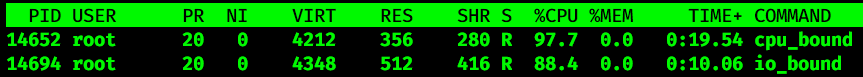
\includegraphics[width=\linewidth]{exp1_top.png}
        \caption{任务一程序资源占用情况}
    \end{figure}
    \paragraph{结果分析:}\quad\par
    从top命令我们可以看到,\bash{cpu_bound}比\bash{io_bound}的cpu占用率高很多。这是因为\bash{io_bound}有大量的I/O操作,导致CPU空闲时间比较长。
    而\bash{cpu_bound}的工作全部是计算,所以CPU使用率很高。
    \section{总结与体会}
FUC*K U SEU :)
\end{document}